\documentclass[conference]{IEEEtran}
\usepackage[utf8]{inputenc}
\usepackage{graphicx}
\usepackage{amsmath}
\usepackage{amssymb}
\usepackage{hyperref}
\usepackage{cite}
\usepackage{booktabs}
\usepackage{algorithm}
\usepackage{algpseudocode}
\usepackage{etoolbox}
\hypersetup{hidelinks}
\usepackage{enumitem}
\setlist[itemize]{leftmargin=1.3em,itemsep=2.5pt,topsep=3pt,parsep=0pt}

% Moderate vertical spacing (readable, not over-compressed)
\renewcommand{\topfraction}{0.96}
\renewcommand{\dbltopfraction}{0.96}
\renewcommand{\bottomfraction}{0.7}
\renewcommand{\textfraction}{0.04}
\renewcommand{\floatpagefraction}{0.85}
\renewcommand{\dblfloatpagefraction}{0.85}
\setcounter{topnumber}{3}
\setcounter{dbltopnumber}{3}
\setcounter{totalnumber}{5}
\setlength{\textfloatsep}{7pt plus 2pt minus 2pt}
\setlength{\dbltextfloatsep}{8pt plus 2pt minus 2pt}
\setlength{\floatsep}{7pt plus 2pt minus 2pt}
\setlength{\intextsep}{7pt plus 2pt minus 2pt}
\setlength{\abovedisplayskip}{4pt plus 1pt minus 1pt}
\setlength{\belowdisplayskip}{4pt plus 1pt minus 1pt}
\setlength{\abovedisplayshortskip}{3pt}
\setlength{\belowdisplayshortskip}{3pt}
% Mild bibliography spacing (font unchanged, readable)
\let\WLDthebibliography\thebibliography
\renewcommand\thebibliography[1]{\WLDthebibliography{#1}%
  \setlength{\itemsep}{0pt}\setlength{\parsep}{0pt}}
\usepackage{tikz}
% ---- Morandi / pastel palette (containers 4-6%, accents muted) ----
\definecolor{ctSlate}{HTML}{F0F4F8}   % data / construction container
\definecolor{ctSage}{HTML}{F2F7F4}    % selection / gating container
\definecolor{ndIce}{HTML}{DCE8F2}     % physics-baseline nodes
\definecolor{ndAmber}{HTML}{F7E6C4}   % evidence gate fill
\definecolor{lnAmber}{HTML}{B98B2E}   % evidence gate stroke
\definecolor{lnSage}{HTML}{4E7C5B}    % gate signal
\definecolor{lnSlate}{HTML}{40566B}   % structural strokes
\definecolor{ndWarm}{HTML}{FAF1E4}    % learned-model tint
\definecolor{ndMint}{HTML}{E7F1EA}    % admitted branch tint
\definecolor{Accent}{HTML}{B35A00}     % single accent used in all figures
\usetikzlibrary{positioning,arrows.meta,fit,backgrounds,calc}

% Horizontal justification for table notes
\patchcmd{\table}{\refstepcounter{table}}{\refstepcounter{table}}{}{}

% Pack floats tighter (workshop page budget)
\renewcommand{\topfraction}{0.95}
\renewcommand{\dbltopfraction}{0.95}
\renewcommand{\textfraction}{0.05}
\renewcommand{\floatpagefraction}{0.85}
\renewcommand{\dblfloatpagefraction}{0.85}
\setcounter{topnumber}{3}
\setcounter{dbltopnumber}{3}
\setcounter{totalnumber}{4}

\setlength{\textfloatsep}{7pt plus 2pt minus 2pt}
\setlength{\floatsep}{6pt plus 2pt minus 2pt}
\setlength{\intextsep}{6pt plus 2pt minus 2pt}
\setlength{\dbltextfloatsep}{7pt plus 2pt minus 2pt}
\setlength{\dblfloatsep}{6pt plus 2pt minus 2pt}
\setlength{\abovecaptionskip}{3pt}
\setlength{\belowcaptionskip}{0pt}

\begin{document}

\title{Evidence-Gated Residual Doppler Correction for LR-FHSS
Direct-to-Satellite IoT}

\author{
\IEEEauthorblockN{
\begin{tabular}{ccc}
Anonymous Author 1 & Anonymous Author 2 & Anonymous Author 3
\end{tabular}}
\IEEEauthorblockA{
\begin{tabular}{ccc}
\begin{tabular}{c}Affiliation omitted for\\double-blind review\\Email omitted\end{tabular} &
\begin{tabular}{c}Affiliation omitted for\\double-blind review\\Email omitted\end{tabular} &
\begin{tabular}{c}Affiliation omitted for\\double-blind review\\Email omitted\end{tabular}
\end{tabular}}
}

\maketitle

\begin{abstract}
Direct-to-Satellite (D2S) IoT terminals pre-compensate LEO Doppler for every
LR-FHSS uplink using stale orbital elements propagated by SGP4. Learning a
residual correction on top of that baseline raises a deployment question rather
than a modelling one: a measurable prediction gain need not be reliable, nor
operationally useful. We present an \emph{evidence-gated} residual correction
framework: inter-TLE residuals are turned into a supervised target, a
low-capacity candidate family is fitted, and the learned branch is admitted only
when a strictly later validation window improves on the physics baseline by a
predefined margin. Using model-derived Space-Track element histories for nine
LEO objects spanning five orbital regimes and six staleness bands from 8 to
168~h, the gate opens in none of 54 target-specific configurations, and limited
BLACK~KITE cross-direction checks likewise remain closed. A five-threshold
residual-screening study yields exactly one opening among 270 configurations,
and that opening is not robust to adjacent thresholds. Residual structure is
nevertheless detectable: an IRIDIUM case shows a reproducible $\approx1.9\%$
held-out improvement that survives multiplicity and temporal diagnostics. Its
absolute size is $3.3$~mHz, against a $500$~Hz control tolerance that lies $917$
residual standard deviations away, and it yields no resolvable endpoint-budget
benefit. These results separate statistical detectability, deployment margin and
endpoint value. All references are later-TLE SGP4 propagations rather than
measured Doppler; no packet-level or over-the-air performance is claimed.
\end{abstract}

\begin{IEEEkeywords}
Direct-to-Satellite IoT, LR-FHSS, endpoint control, stale TLE, SGP4, inter-TLE
residual, validation-gated deployment, LEO satellite
\end{IEEEkeywords}

\section{Introduction}
\label{sec:intro}

Direct-to-Satellite (D2S) IoT over Low-Earth Orbit (LEO) connects
power-constrained end devices without terrestrial infrastructure, but the high
relative velocity induces Doppler shifts of order $20$~kHz at 868~MHz and rapid
Doppler-rate changes that stress the physical layer~\cite{hurn2023lrfhss}.
Long-Range Frequency-Hopping Spread Spectrum
(LR-FHSS)~\cite{semtech2023lrfhss} spreads transmit energy across narrow
frequency bins, so residual frequency error after pre-compensation widens the
guard the terminal must reserve, raises the chance of missing a hop bin, and
spends airtime a battery-powered node cannot recover.

The terminal must size these margins \emph{before} transmitting, from a
\emph{stale} TLE propagated open-loop by SGP4/SDP4~\cite{hoots1980models}. That
baseline is already strong: the inter-TLE frequency residual it leaves is well
under one Hz at short staleness. Whether a learned corrector improves on it is
usually settled by measuring a prediction gain. We argue that this is the wrong
test, and that three criteria must be kept apart:
\begin{equation}
\underbrace{\text{detectability}}_{\text{is the gain real?}}
\;\neq\;
\underbrace{\text{margin}}_{\text{large enough?}}
\;\neq\;
\underbrace{\text{endpoint value}}_{\text{changes the budget?}}
\label{eq:axes}
\end{equation}
A corrector can satisfy the first and fail the other two, and deploying on the
first alone is what an always-on learned branch does. We therefore study the
pre-transmission decision directly, formalised as an \emph{Evidence Gate}: a
learned residual is admitted only when a chronological, leakage-free validation
window beats the physics baseline by a predefined margin~$\gamma$, and SGP4 is
retained otherwise, on real Space-Track element histories for nine LEO objects
across five orbital regimes.

\emph{Related work.} Prior art spans link, capacity and energy analyses of
aggregate LR-FHSS behaviour under LEO Doppler and
load~\cite{semtech2023lrfhss,ullah2022lrfhss,hurn2023lrfhss}; synchronisation and
pre-compensation, from NTN timing advance and ToA/CFO
estimation~\cite{3gpp2019tr38821} to endpoint Doppler pre-compensation driven by
a satellite-broadcast beacon~\cite{ullah2025precomp}; and orbit learning, which
corrects SGP4/SDP4~\cite{hoots1980models} trajectories for trajectory
accuracy~\cite{peng2019gp,acciarini2025dsgp4,caldas2024mlorbit}, while D2S uplink
policies~\cite{alvarez2022uplink} choose \emph{when} to transmit given a
prediction assumed trustworthy. The closest,~\cite{ullah2025precomp}, also
pre-compensates at the end device but estimates the shift from a downlink beacon;
we assume no downlink and correct open-loop from a stale element set, so our
question is not how to estimate the shift but whether a learned correction to it
may be trusted. None decides, before transmission, whether a learned residual
should be trusted. Contributions:
\begin{itemize}
\item \emph{Evidence-gated residual correction framework.} A software method
that constructs inter-TLE residual targets, fits a nested candidate family, and
admits the learned branch only when a chronological validation margin is met,
retaining SGP4 otherwise (Sec.~\ref{sec:method}).
\item \emph{Multi-regime real-data evaluation.} Across nine LEO objects, five
regimes and six staleness bands, no branch earns deployment at the pre-specified
operating point; a five-threshold screening analysis yields one isolated,
non-robust opening (Secs.~\ref{sec:res-primary}--\ref{sec:res-screen}).
\item \emph{Learnability-to-value diagnosis.} A reproducible $\approx1.9\%$
IRIDIUM gain is $3.3$~mHz of absolute correction with no resolvable
endpoint benefit, separating the three criteria of Eq.~\eqref{eq:axes}
(Sec.~\ref{sec:res-value}).
\end{itemize}

\section{System Model and Evidence-Gated Correction}
\label{sec:method}

\begin{figure*}[!t]
\centering
\resizebox{\textwidth}{!}{%
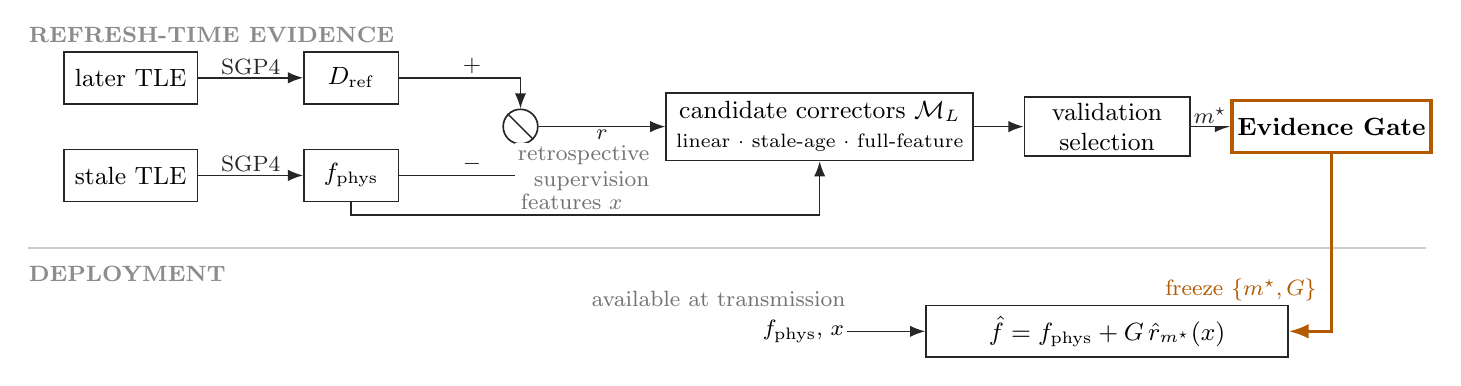
\begin{tikzpicture}[
  x=1cm, y=1cm, font=\small, >=Latex,
  b/.style={draw=black!85, line width=0.6pt, align=center, minimum height=6.6mm,
            minimum width=17mm, inner sep=2pt, fill=white},
  q/.style={b, minimum width=12mm},
  ml/.style={b, minimum width=39mm, minimum height=8.6mm},
  ga/.style={b, draw=Accent, line width=1.3pt, minimum width=23mm},
  sj/.style={draw=black!85, line width=0.6pt, circle, inner sep=0pt,
             minimum size=4.4mm, fill=white},
  ar/.style={->, line width=0.55pt, black!85},
  % white knockout behind short labels so strokes never cross glyphs
  sig/.style={font=\footnotesize, inner sep=1pt, fill=white},
  tag/.style={font=\footnotesize, text=black!55, inner sep=1pt, fill=white},
  ph/.style={font=\footnotesize\bfseries, text=black!45, inner sep=0pt}]

% ================= phase 1: refresh-time evidence =================
\node[ph, anchor=west] at (0.05, 2.16) {REFRESH-TIME EVIDENCE};

\node[b] (lt) at (1.35, 1.62) {later TLE};
\node[b] (st) at (1.35, 0.38) {stale TLE};
\node[q] (dr) at (4.15, 1.62) {$D_{\mathrm{ref}}$};
\node[q] (fp) at (4.15, 0.38) {$f_{\mathrm{phys}}$};
\draw[ar] (lt) -- node[sig, above] {SGP4} (dr);
\draw[ar] (st) -- node[sig, above] {SGP4} (fp);

% subtraction junction on the main baseline: D_ref (+) minus f_phys (-)
\node[sj] (sj) at (6.30, 1.00) {};
\draw[line width=0.5pt, black!85] (sj.north west) -- (sj.south east);
\draw[ar] (dr.east) -| node[sig, pos=0.30, above] {$+$} (sj.north);
\draw[ar] (fp.east) -| node[sig, pos=0.30, above] {$-$} (sj.south);

\node[ml] (cand) at (10.10, 1.00)
  {candidate correctors $\mathcal{M}_L$\\[-0.5pt]\scriptsize linear $\cdot$ stale-age $\cdot$ full-feature};
\draw[ar] (sj.east) -- node[sig, below] {$r$} (cand.west);
\node[tag, anchor=north east, align=right] at (7.98, 0.80)
  {retrospective\\supervision};

% feature path: independent of r, own lane above the divider
\draw[ar] (fp.south) -- (4.15,-0.12) -- (10.10,-0.12) -- (cand.south);
\node[tag, anchor=south] at (6.95,-0.09) {features $x$};

\node[b, minimum width=21mm] (sel) at (13.75, 1.00) {validation\\selection};
\draw[ar] (cand) -- (sel);
\node[ga] (gate) at (16.60, 1.00) {\textbf{Evidence Gate}};
\draw[ar] (sel) -- node[sig, above] {$m^{\star}$} (gate);

% ================= phase 2: frozen deployment =================
\draw[black!20, line width=0.5pt] (0.05,-0.54) -- (17.80,-0.54);
\node[ph, anchor=west] at (0.05,-0.87) {DEPLOYMENT};

\node[b, minimum width=46mm] (out) at (13.75,-1.60)
  {$\hat f = f_{\mathrm{phys}} + G\,\hat r_{m^{\star}}(x)$};
\node[sig, anchor=east] (in) at (10.45,-1.60) {$f_{\mathrm{phys}},\,x$};
\node[tag, anchor=south east] at (10.47,-1.33) {available at transmission};
\draw[ar] (in.east) -- (out.west);
\draw[ar, Accent, line width=0.9pt] (gate.south) -- (16.60,-1.60) -- (out.east);
\node[sig, text=Accent, anchor=east] at (16.45,-1.07) {freeze $\{m^{\star},G\}$};
\end{tikzpicture}}
\caption{Evidence-gated residual correction. \emph{Refresh time:} a later element
and the stale element in use are each propagated by SGP4, and the subtraction
junction forms the retrospective residual target of Eq.~\eqref{eq:residual};
because the later element does not exist at the original transmission, $r$
supervises only correctors applied to subsequent transmissions. With the feature
vector $x$ it drives the candidate set $\mathcal{M}_L$, from which validation selects
$m^{\star}$; the Evidence Gate then compares that branch's validation error with
the physics baseline's, $\mathrm{MAE}_{m^{\star}}(V)<\gamma\,\mathrm{MAE}_{\mathrm{phys}}(V)$,
and freezes $\{m^{\star},G\}$. \emph{Deployment:} the frozen state is applied
without refitting or re-gating. The split, screening rule and diagnostic reference
predictors are in Sec.~\ref{sec:data} and Algorithm~\ref{alg:gate}.}
\label{fig:architecture}
\end{figure*}

\subsection{Doppler, Stale TLE and the Inter-TLE Residual}
In a LEO pass the one-way Doppler is $f_D(t) = -\,v_r(t)\,f_c/c$, with $v_r$ the
radial velocity, and the residual carrier-frequency error after
pre-compensation is
\begin{equation}
f_{\mathrm{res}}(t) = f_D(t) - \hat{f}_D(t) + f_{\mathrm{osc}},
\label{eq:residual_cfo}
\end{equation}
where $\hat f_D$ is the prediction and $f_{\mathrm{osc}}$ the oscillator offset.
Equation~\eqref{eq:residual_cfo} separates the orbital-prediction term from
endpoint RF errors, which can dominate the absolute residual; only the
TLE-driven component is isolated here. Reliable hop reception is modelled as
$|f_{\mathrm{res}}|$ staying small relative to a tolerance
$F_{\mathrm{tol}}$---a control proxy, not a standard-compliant receiver model.

The terminal holds a TLE older than the present epoch; propagating it with SGP4
gives the deployable prediction $f_{\mathrm{phys}}(t)$. We define a
model-derived \emph{reference} $D_{\mathrm{ref}}(t)$ as the SGP4 propagation of
a \emph{later} element set for the same object at the same UTC---a newer orbit
solution, not an RF measurement. The residual
\begin{equation}
r(t) = D_{\mathrm{ref}}(t) - f_{\mathrm{phys}}(t)
\label{eq:residual}
\end{equation}
is what a TLE-only terminal can observe by comparing element sets; it encodes
mean-element updates, drag-term changes and fit differences. The reference is not
available while the stale element is in use, so $r(t)$ is \emph{retrospective}
supervision: computable only once the later element is published, and used to
train correctors applied to \emph{subsequent} transmissions. A learned corrector
forms $f_{\mathrm{ml}}(t)=f_{\mathrm{phys}}(t)+\hat r(x_t)$ from a feature
vector $x_t$ described in Sec.~\ref{sec:models}.

\subsection{The Evidence Gate}
\label{sec:gate}
Let $V$ be a chronological validation window, strictly later than the training
span and strictly earlier than the held-out test span, so no future element set
leaks into model selection. On $V$ we measure the mean absolute frequency error
of both branches, $\mathrm{MAE}_{\mathrm{phys}}(V)$ and
$\mathrm{MAE}_{\mathrm{ml}}(V)$, and admit learning only on a proven margin,
\begin{equation}
G = \mathbf{1}\!\left[\,\mathrm{MAE}_{\mathrm{ml}}(V) < \gamma\,
\mathrm{MAE}_{\mathrm{phys}}(V)\,\right],\qquad \gamma\in(0,1],
\label{eq:gate}
\end{equation}
deploying $\hat f = G f_{\mathrm{ml}} + (1-G) f_{\mathrm{phys}}$.
Figure~\ref{fig:architecture} places this decision inside the surrounding
software method; Algorithm~1 states the full procedure. Training fits the candidates; validation both selects
the candidate and decides $G$; the held-out segment reports the consequence of
that already-frozen policy and never selects a model or decides the gate. By
construction the gate gives a validation-window property, not a
distribution-shift bound. We use $\gamma=0.95$, a conservatism setting fixed in
a version-controlled protocol before any result was inspected, and report
sensitivity in Sec.~\ref{sec:res-value}.

\begin{algorithm}[t]
\caption{Evidence-Gated Residual Deployment}
\label{alg:gate}
\begin{algorithmic}[1]
\Require canonical history $H$; staleness target $\tau$; \emph{learned}
candidate set $\mathcal{M}_L$; margin $\gamma$; screen $\tau_s$
\State $P \gets \textsc{BuildPairs}(H,\tau)$
\Comment{stale/reference pairs, $K$ samples each}
\State $P \gets \textsc{Screen}(P,\tau_s)$
\Comment{drop pairs with $\max|r|>\tau_s$}
\State $T,V,E \gets \textsc{ChronologicalSplit}(P)$
\Comment{by reference epoch, $60/20/20$}
\ForAll{$m \in \mathcal{M}_L$}
  \State $\textsc{Fit}(m,T)$;\quad $J_m \gets \mathrm{MAE}(m,V)$
\EndFor
\State $m^{\star} \gets \arg\min_{m \in \mathcal{M}_L} J_m$
\Comment{references never compete}
\State $G \gets \mathbf{1}[\,J_{m^{\star}} < \gamma\,\mathrm{MAE}_{\mathrm{phys}}(V)\,]$
\State $\textsc{Freeze}(m^{\star},G)$
\Comment{policy is now immutable}
\State \textbf{report} $\textsc{Evaluate}(m^{\star},G,E)$
\Comment{$E$ is queried only here}
\end{algorithmic}
\end{algorithm}

The held-out set $E$ is not queried at any point before line~9; no quantity
derived from $E$ enters $\arg\min$, the margin test, or hyper-parameter choice.
This is checked mechanically (Sec.~\ref{sec:stats}).

\subsection{When the Gate Is Re-Decided}
\label{sec:semantics}
Fitting and gating are refresh-time operations, not per-transmission ones
(Fig.~\ref{fig:architecture}).

\emph{On a new element set} (median inter-element gap 4.5--10.0~h here) the
residual history is extended, $\mathcal{M}_L$ is refitted on training, and
$m^{\star}$ and $G$ are re-decided on a fresh validation window; only the
corrector, the gate bit and its metadata are persisted.

\emph{Between refreshes} the state is immutable: a transmission applies
$\hat f = f_{\mathrm{phys}} + G\,\hat r_{m^{\star}}(x)$ with no refitting,
selection or gate evaluation. Continuously adapting the corrector would
reintroduce the unaudited, always-on behaviour the gate exists to prevent and
would make the acting policy impossible to attribute afterwards. When evidence
lapses the gate reverts to $G=0$.

\section{Data, Software Pipeline and Evaluation Protocol}
\label{sec:data}

\subsection{Dataset Qualification}
\label{sec:qual}
The acquisition and qualification contract was fixed in a version-controlled
protocol before evaluation and executed before any learner was run. A satellite is \emph{retained} only if at least
$B_{\min}=2$ staleness bands are supported, where a band counts as supported
only when the chronological split yields at least $n_{\min}=3$ pairs in each of
the training, validation and test segments. The dataset qualifies only if at
least $S_{\min}=6$ satellites are retained spanning at least $R_{\min}=3$
distinct orbital regimes, regimes being derived from the ingested elements as
altitude$\,\times\,$inclination cells, not from acquisition intent.

Eleven histories were acquired; nine were retained (Table~\ref{tab:data})
spanning five regimes with all six bands supported. Two newly launched Starlink
objects were excluded because their $\approx4.5$-day histories cannot fill a
chronological split at any band---an insufficient-coverage exclusion decided by
the qualification rule, not by learning performance.

\subsection{Canonical Orbital History}
\label{sec:canonical}
Each object's history is distributed in two encodings of the same solutions. The
JSON element history is the single canonical scientific input; the archival TLE
file is kept for provenance and never ingested as an additional observation set,
since doing so duplicates each solution and collapses the apparent update cadence
toward zero. Epochs are normalised deterministically to a fixed quantum and
grouped by catalogue number and normalised epoch.

Such a group is not automatically a duplicate: Space-Track republishes an epoch
when the solution is re-fitted, and $884$ groups here hold two or more physically
distinct solutions. \emph{Equivalent duplicate collapse} covers only rows agreeing
on mean elements, drag term and ephemeris type and differing in publication
bookkeeping; the rest need \emph{same-epoch revision resolution}, which selects
one solution by publication metadata, never by averaging.

The canonical rule is the \emph{earliest} published revision---an availability
argument, not a performance one. In $237$ of the $884$ groups the last revision
was created only after the \emph{next} element set already existed, so choosing
it would let a terminal correct with a solution that did not yet exist.
Canonicalisation leaves $46\,859$ elements from $52\,538$ raw rows for the
largest object and restores plausible update cadences
(Table~\ref{tab:data}). The retained identifier, creation date and
competing-revision count are recorded for every resolved epoch.

Canonicalisation is not load-bearing: resolving the same groups to the
\emph{latest} revision leaves every headline count unchanged. Deleting all
contested epochs---an ablation, not a rule, since it discards real
observations---opens one configuration, BLACK~KITE-2 at 48~h, whose validation
gain rises to $6.1\%$ while its held-out result is $-4.3\%$ on 37 pairs, with
Holm-adjusted $p=0.52$. That is the validation/test mismatch this paper is
about, not deployable learnability; it is the hollow marker in
Fig.~\ref{fig:multisat}.

\subsection{Pair Construction and Staleness Bands}
\label{sec:pairs}
For each reference (newer) element set we select the older set whose epoch gap
is closest to the staleness target within an admissible band. The six targets
and their bands $[\,\text{lo},\text{hi}\,]$ in hours are
$8\!:\![4,14]$, $24\!:\![16,36]$, $48\!:\![36,60]$, $72\!:\![60,84]$,
$96\!:\![84,120]$ and $168\!:\![144,192]$. Consecutive element sets are not
required: this reproduces the case in which a terminal holds a TLE roughly
$\tau$ hours old. The pair is propagated open-loop and compared to the reference
at $K=24$ UTC samples spanning one orbital period ($5700$~s), at an $868$~MHz
carrier for a representative ground station ($24^\circ$N, $121^\circ$E). A pair is screened out if any of its samples
exceeds $\max|r|>\tau_s$, with $\tau_s=1500$~Hz as the pre-specified value.
Screening is applied \emph{before} the chronological split, so it changes the
population that is split rather than the split boundaries;
Sec.~\ref{sec:res-screen} varies $\tau_s$ explicitly. Splits are $60/20/20$ by
reference epoch, using two global boundaries shared by every band of an object.

\subsection{Residual Candidate Models}
\label{sec:models}
The feature vector $x_t$ has ten entries: TLE age and epoch gap, the stale-TLE
Doppler, $\sin$ and $\cos$ of the orbital phase, elevation and slant range, and
the stale mean motion, drag term and eccentricity. The \emph{learned candidate
set} $\mathcal{M}_L$ holds three fitted correctors; two further predictors are
diagnostic references and never enter selection:
\begin{align}
\mathcal{M}_L:\;\; &\hat r(x_t) = a\,t_{\mathrm{age}} + b,\;\;
  \hat r(x_t) = w^{\!\top} z(t_{\mathrm{age}},t_{\mathrm{gap}}) + w_0,
  \label{eq:models}\\
 &\hat r(x_t) = w^{\!\top} z(x_t) + w_0, \nonumber\\
\text{ref.:}\;\; &\hat r = 0\;(\text{SGP4}),\;\;
  \hat r = c,\; c\in\{\operatorname{mean}(r_T),\operatorname{median}(r_T)\}
  \nonumber
\end{align}
with $z(\cdot)$ standardisation fitted on training and the ridge penalty chosen
from $\{10^{-2},\dots,10^{3}\}$ on validation. Selection runs over $\mathcal{M}_L$
only, $m^{\star}=\arg\min_{m\in\mathcal{M}_L}\mathrm{MAE}_m(V)$: the zero
predictor is the physics baseline the gate compares against and the
constant-bias predictors are diagnostic, so neither competes for $m^{\star}$ nor
can open the gate.

$\mathcal{M}_L$ is deliberately low-capacity: the question is whether
low-dimensional, chronologically stable residual structure exists at all, a
precondition for high-capacity learning to be worth its deployment and audit
burden. Its low capacity limits, rather than eliminates,
validation-window overfitting.

\subsection{Statistical and Deployment Evaluation}
\label{sec:stats}
The independent experimental unit is the accepted TLE pair, never the individual
propagation sample: the $K=24$ samples within a pair are one propagation over one
orbit and are strongly correlated. Every metric is computed per pair then
averaged, and every statistic is paired at pair level. We report the pair-level MAE, the learned win fraction, an exact two-sided sign
test, a bootstrap interval resampling pair identifiers, a block bootstrap
resampling whole reference-epoch days to respect dependence between adjacent
pairs, and Holm-adjusted $p$-values across the family of tests.

These statistics are diagnostics and never modify the deployment decision: $G$
depends only on the margin test of Eq.~\eqref{eq:gate}, so a result can be
strongly significant and still refused, and a marginal one is never promoted for
a small $p$-value. Keeping the two separate is the point of Eq.~\eqref{eq:axes}.

Before any result is emitted the pipeline asserts mechanically that train,
validation and test pair identifiers are disjoint, that validation strictly
precedes test, that one accepted pair contributes exactly one observation, and
that $G$ is reproducible from validation quantities alone.

\emph{Endpoint mapping.} To convert a residual into terminal cost we use control
proxies: a guard proxy $g = 2\,p_{99}(|e|)$ on the error $e$ of whichever branch
the gate selects, an outage proxy $\rho=\Pr[|e|>F_{\mathrm{tol}}]$ with a
representative sub-kHz tolerance $F_{\mathrm{tol}}=500$~Hz---a modelling choice,
not an LR-FHSS conformance requirement---and, treating timing and frequency
misses as independent, a joint success proxy and energy per burst
\begin{equation}
S=(1-P_t)(1-P_f),\quad
E_{\mathrm{succ}} = \frac{I_{\mathrm{rx}}V(g_t+t_{\mathrm{rx}})
+P_{\mathrm{tx}}t_{\mathrm{tx}}}{S},
\label{eq:esucc}
\end{equation}
with $P_f=\operatorname{erfc}\!\big(F_{\mathrm{tol}}/(\sigma_{\mathrm{res}}
\sqrt2)\big)$, $\sigma_{\mathrm{res}}$ the held-out residual standard deviation,
$g_t=g_0+3\sigma_t$ the timing guard and $\sigma_t$ mapped from TLE age.
Parameters follow the analysis scripts ($g_0=30$~ms, $t_{\mathrm{rx}}=50$~ms at
$12$~mA/$3.3$~V, $14$~dBm for $t_{\mathrm{tx}}=200$~ms). These are control-layer
proxies for margin sizing, not packet-error, bit-error or link-budget
measurements.

\begin{table}[t]
\centering
\footnotesize
\caption{The nine retained objects. Elements are canonical solutions after
equivalent-duplicate collapse and same-epoch revision resolution; all six
staleness bands are supported for every object. Eleven histories were acquired
and two were excluded for insufficient chronological coverage. All values are
model-derived from element sets, not measured.}
\label{tab:data}
\setlength{\tabcolsep}{3.2pt}
\begin{tabular}{llrrrr}
\toprule
Object & Regime (alt.\,/\,incl.) & Alt. & Incl. & Elem. & Gap \\
 & & [km] & [$^\circ$] & & [h] \\
\midrule
ISS (ZARYA)   & very low / mid-incl. & 388  & 51.6 & 46\,859 & 4.52 \\
FLOCK 4H 1    & low / SSO            & 507  & 97.4 & 614     & 7.89 \\
FLOCK 4H 2    & low / SSO            & 507  & 97.4 & 635     & 7.89 \\
BLACK KITE-1  & low / SSO            & 507  & 97.4 & 446     & 6.33 \\
BLACK KITE-2  & low / SSO            & 590  & 97.8 & 252     & 8.04 \\
IRIDIUM 177   & mid / near-polar     & 629  & 86.2 & 2\,623  & 9.73 \\
IRIDIUM 181   & high / near-polar    & 743  & 86.6 & 2\,678  & 9.98 \\
ONEWEB-0015   & upper / near-polar   & 1114 & 87.7 & 1\,695  & 8.00 \\
SENTINEL-6B   & upper / mid-incl.    & 1336 & 66.0 & 727     & 5.62 \\
\bottomrule
\end{tabular}
\end{table}

% ── Results ──────────────────────────────────────────────────────────────────
\section{Results}
\label{sec:results}

\begin{figure*}[!t]
    \centering
    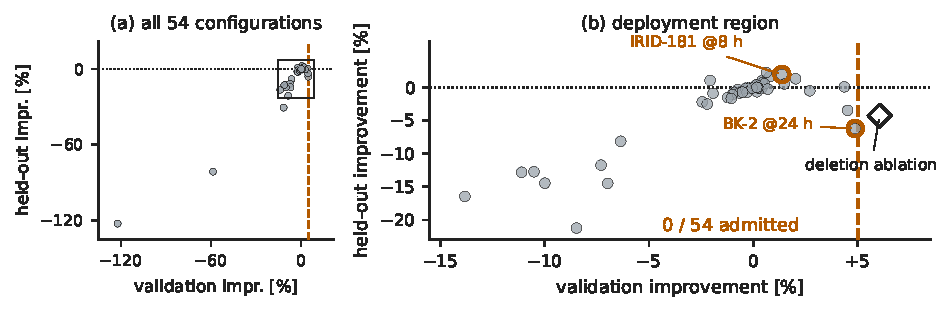
\includegraphics[width=\textwidth]{figures_final/fig_decision_map.pdf}
    \caption{What validation told the gate, and what happened next, for all 54
    target-specific configurations at the pre-specified operating point
    ($\gamma=0.95$, 1500~Hz screen). Positive means the learned branch is better on
    both axes. (a)~All configurations at true coordinates; outcomes are strongly
    heterogeneous, ONEWEB-0015 at 24~h reaching $-122\%$ on both axes, and the
    rectangle marks the region enlarged in~(b). (b)~The gate reads only the
    horizontal axis and admits a branch beyond the dashed $+5\%$ margin, which
    \textbf{0 of 54} reach; the nearest miss is BLACK~KITE-2 at 24~h ($+4.9\%$
    validation, $-6.2\%$ held-out). The hollow diamond is the non-canonical
    conflict-deletion ablation of Sec.~\ref{sec:canonical}, the only configuration
    that crosses the margin under any canonicalisation setting tested, and
    harmful on held-out data when it does.
    Cross-direction continuity opens 0 of 12; residuals are model-derived
    inter-TLE differences, not measured Doppler.}
\label{fig:multisat}
\end{figure*}

\subsection{Multi-Satellite Deployment Result}
\label{sec:res-primary}
Figure~\ref{fig:multisat} reports the 54 target-specific configurations. No
learned correction earns deployment at the pre-specified operating point: the
gate is closed in every object and band, and the limited BLACK~KITE
cross-direction checks are closed in all 12. We do not claim a complete
cross-satellite transfer matrix.

The held-out consequences are heterogeneous even though the decision is not.
SENTINEL-6B degrades by $8$--$31\%$ at every band and ONEWEB-0015 by up to
$122\%$, while ISS moves by less than $0.4\%$ anywhere and both IRIDIUM objects
improve slightly at several bands. The refusal is uniform not because harm is, but
because no branch clears the validation margin.

The screened fraction grows with staleness, from under $0.3\%$ at 8~h to $28.5\%$
for ISS and $16.9\%$ for ONEWEB-0015 at 168~h, as longer propagation exposes
manoeuvre and bad orbit-determination epochs. Effect size and resolution are also
misaligned: ISS contributes 14\,000--19\,000 held-out pairs per band, so its
$0.1\%$ degradations are overwhelmingly significant, while SENTINEL-6B reaches
$31\%$ on 131 pairs. The gate, a margin rather than a $p$-value, is unaffected.

\subsection{Detectable but Sub-Margin Residual Structure}
\label{sec:res-detect}
A refusal is only informative if the learner can find structure where it exists.
It can. For IRIDIUM~181 at 8~h the validation-selected corrector reduces held-out
pair-level MAE from $0.16740$ to $0.16414$~Hz, a $1.94\%$ improvement winning on
$61.8\%$ of 633 pairs (Fig.~\ref{fig:axes}(a)). It survives Holm correction and a
day-blocked bootstrap, has a bootstrap $95\%$ interval of $[-4.1,-2.4]$~mHz
excluding zero, and---unlike most signals here---keeps its sign at every screen
(Fig.~\ref{fig:axes}(b)). Comparable sub-margin gains appear for IRIDIUM~177 at 96
and 168~h, and the stale-age ridge is selected in every such cell, consistent with
the correction tracking element staleness rather than pass geometry.

The gate nonetheless stays closed: the validation gain is $1.37\%$ against the
$5\%$ that $\gamma=0.95$ requires---a deployment margin working as intended, not
a missed detection. Reporting only the relative gain, as a prediction-accuracy
study would, would have made this cell look deployable.

\subsection{Screening Robustness}
\label{sec:res-screen}
Because the residual screen removes outlier pairs, it could in principle
manufacture either conclusion. We re-executed the pipeline independently at
none, 150, 500, 1500 and 3000~Hz, refitting and re-gating at each: 270
configurations.

Exactly \textbf{one} of the 270 opens: IRIDIUM~177 at 168~h under the 150~Hz
screen, which discards $40.3\%$ of candidate pairs. Adjacent thresholds contradict
it, its Holm-adjusted $p$ is $1.00$, and it is not the pre-specified operating
point (Fig.~\ref{fig:axes}(b)).

Comparing no screening against the pre-specified rule across all 54 cells,
screening improves the learned branch's relative performance in 36, worsens it in
4 and leaves 14 unchanged---all cells where it removes no pairs---with a median
shift of $1.26$ percentage points in its favour. The aggregate direction is
inconsistent with the 1500~Hz screen manufacturing the negative result;
training-composition and evaluation-membership effects are not causally separated.

\begin{figure*}[!t]
    \centering
    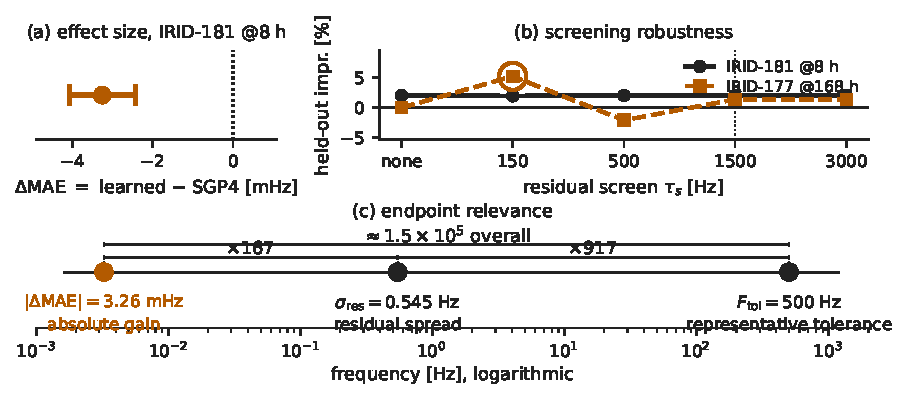
\includegraphics[width=0.98\textwidth]{figures_final/fig_evidence_axes.pdf}
    \caption{Three criteria on the same effect. (a)~Pair-level effect size for
    IRIDIUM~181 at 8~h: point estimate and $95\%$ pair-bootstrap interval over
    $n=633$ held-out pairs, with the learned branch better on $61.8\%$ of them; the
    effect survives Holm correction and a day-blocked bootstrap. (b)~That sign
    holds at every screening threshold, whereas the single IRIDIUM~177 opening at
    150~Hz (hollow marker; the only opening among 270 configurations,
    Holm-adjusted $p=1.00$) is contradicted by its neighbours; the dotted line is
    the pre-specified screen. (c)~The same gain against the endpoint scale. The
    three quantities are not interchangeable: they are the absolute size of the
    correction, the spread of the residual it acts on, and a representative control
    tolerance. All endpoint quantities are software control proxies.}
\label{fig:axes}
\end{figure*}

\subsection{Deployment Margin versus Endpoint Value}
\label{sec:res-value}

No cell in Fig.~\ref{fig:multisat} produces a resolvable endpoint change, because
the decisive comparison is relative against absolute scale: the IRIDIUM~181
improvement is $1.94\%$ relative but $3.26$~mHz absolute, against
$F_{\mathrm{tol}}=500$~Hz. With $\sigma_{\mathrm{res}}=0.545$~Hz the tolerance
lies $917$ residual standard deviations away, so the frequency-miss term of
Eq.~\eqref{eq:esucc} is $\log_{10}P_f<-1.8\times10^{5}$ for both branches. The
guard proxy moves from $4.470$ to $4.439$~Hz, $2.3\times10^{-7}$ of the hopping
bandwidth; the outage proxy is zero for both; and $S$ and $E_{\mathrm{succ}}$ are
indistinguishable at double precision, both $15.94$~mJ per burst
(Fig.~\ref{fig:axes}(c)). A $30.7\%$ \emph{degradation} for SENTINEL-6B is
likewise endpoint-invisible, which is why relative MAE alone is a poor indicator
of endpoint relevance.

\emph{Margin sensitivity.} Recomputing the gate at
$\gamma\in\{1.00,0.99,0.98,0.975,0.95,0.90\}$ gives $24, 7, 5, 4, 0, 0$ openings, of
which $16, 4, 2, 1, -, -$ improve on held-out data. Tightening the margin does
\emph{not} monotonically improve held-out selection precision, which falls from
$66.7\%$ to $25.0\%$ before openings vanish; what falls monotonically is the number
of harmful deployments, 8 to 0.

% ── Discussion ───────────────────────────────────────────────────────────────
\section{Discussion, Limitations and Conclusion}
\label{sec:conclusion}

The substantive finding is the separation in Eq.~\eqref{eq:axes}: residual
structure \emph{is} detectable---the IRIDIUM~181 result survives multiplicity,
temporal dependence and screening variation---yet it is sub-margin and leaves the
endpoint budget unchanged. A policy deploying on detectability alone would have
accepted a branch with no resolvable benefit, its deployment burden and its
exposure to distribution shift.

\emph{Design implications.} Three consequences follow. First, statistical
significance is not the deployment criterion: the IRIDIUM~181 effect is
significant under every test we applied and is still refused, because deployment
turns on the margin a branch clears before commitment, not the $p$-value it
attains afterwards. Second, the durable signal is selected by the stale-age ridge
wherever it appears, pointing to a low-dimensional ageing bias rather than
unexploited pass geometry; but its \emph{absolute} size---$3.26$~mHz against a
$0.545$~Hz residual spread---does not justify higher-capacity models. Third, the
deletion ablation exposes the gate's limit: contested-epoch removal lifts one
BLACK~KITE-2 cell across $\gamma$ on validation, yet it loses $4.3\%$ held out.
The margin is an evidential filter, not a guarantee of held-out benefit.

\emph{Limitations.} All results are software-only and model-derived: every
reference is a later element solution propagated by SGP4, not measured Doppler,
and no live-satellite contact, LR-FHSS decoding, error-rate or
gateway-acknowledgement result is claimed. The endpoint budget is a control proxy
depending on the representative $F_{\mathrm{tol}}=500$~Hz, though the
\emph{relative} statement survives plausible re-choices. Nine objects do not
represent all LEO spacecraft, the cross-direction checks are a continuity test
rather than a transfer matrix, and screening effects on training and evaluation
membership were not decomposed. One feature, the stale-to-reference epoch gap, is
fixed by the reference element's publication time and is therefore not computable
at the transmission epoch; two of the three candidates consume it, so the
selections reported here characterise attainable residual structure rather than a
branch a terminal could evaluate unaided. Validation is reused
for ridge-penalty tuning, candidate selection and the gate test, so the margin is
selection-conditioned and that reuse favours the learned branch; the held-out
segment is touched by none of the three. Packet-level and then authorized
over-the-air measurement remain future work.

\emph{Reproducibility.} Qualification, canonicalisation, the pair-level protocol,
all 54 primary and 270 screening configurations, the $\gamma$ frontier and the
endpoint proxies are produced by version-controlled scripts from committed
artifacts, with raw archives held outside the repository under a per-object SHA256
manifest. Figures are rendered from those frozen artifacts.

\emph{Conclusion.} A validation-gated endpoint policy retains the SGP4 baseline
everywhere at the pre-specified operating point, and the most robust detectable
residual correction is worth $3.3$~mHz on a budget that cannot resolve it. The
contribution is not that learning fails, but that three questions usually
collapsed into one---is the gain real, is it large enough, is it worth anything at
the endpoint---have different answers on the same data, and that a gate can ask
the second before paying for the third.

% ── References ───────────────────────────────────────────────────────────────
\IEEEtriggeratref{99}
\IEEEtriggercmd{\relax}
\bibliographystyle{IEEEtran}
\bibliography{refs}

\end{document}
